\chapter{A faster graph search can preserve the wrong relationship}
\label{repair29:discovery}

Before a bank asks whether a higher deposit rate attracts balances, it must
distinguish the effect of changing the rate from the information that led it
to offer that rate. A graph search can help compare explanations, but its
computational shortcuts have scientific consequences. A link retained because
the search stopped is a different finding from a relationship that survived
the relevant tests.

The previous software comparison identified a concrete difficulty in the
inspected Aitiotita revision. Beyond conditioning depth two, one skeleton-search
path tests a pair conditional on the union of its neighbours. If dependence
persists, it marks the link undeletable and omits subsequent subset searches.
That rule would be safe only if dependence after adding variables excluded
independence under a smaller conditioning set. The retained generic callback
allows independence procedures for which that implication fails.
\citep{repair29pc}

This chapter examines a repair: continue the declared subset search, and
report an unfinished search explicitly when its budget is exhausted. The
calculations compare project implementations with exact independence oracles.
They do not execute the Java distribution. The distinction matters because
the inspected bundled linguistic oracle is not a Gaussian test, and the
orientation and graph-export stages require separate evaluation.

\section{A common consequence can undo a valid comparison}

Consider a hypothetical one-period decision. Let $X$ be a rate concession,
$Y$ a subsequent balance response and $Z_1,Z_2,Z_3$ three measured factors
known before the decision. The variables are centred model units; their
coefficients are stipulated, not bank estimates. Each baseline factor affects
both the offered rate and the balance. After the outcome, a score $C$ summarises
the concession and balance response. It is a common consequence, rather than
an additional baseline cause.

\begin{figure}[htbp]
\centering
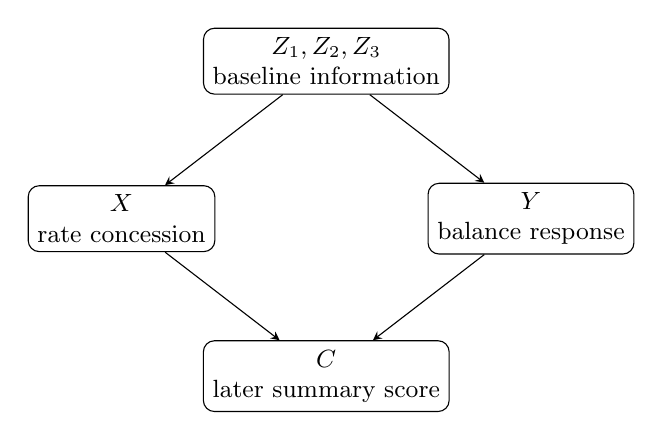
\begin{tikzpicture}[>=stealth, every node/.style={font=\small}]
\node[draw,rounded corners,align=center] (z) at (0,2) {$Z_1,Z_2,Z_3$\\baseline information};
\node[draw,rounded corners,align=center] (x) at (-2.6,0) {$X$\\rate concession};
\node[draw,rounded corners,align=center] (y) at (2.6,0) {$Y$\\balance response};
\node[draw,rounded corners,align=center] (c) at (0,-2) {$C$\\later summary score};
\draw[->] (z)--(x);\draw[->] (z)--(y);
\draw[->] (x)--(c);\draw[->] (y)--(c);
\end{tikzpicture}
\caption{Each baseline factor points to both $X$ and $Y$; the box groups the
three factors for readability. There is no causal arrow from $X$ to $Y$ in
this constructed example. Conditioning on their later common consequence
$C$ nevertheless makes their residuals associated.}
\label{repair29:collider}
\end{figure}

Let all six inputs $Z_1,Z_2,Z_3,\varepsilon_X,\varepsilon_Y,\varepsilon_C$
be mutually independent standard normal variables. The structural equations
are
\begin{align}
X&=Z_1+Z_2+Z_3+\varepsilon_X,\\
Y&=Z_1+Z_2+Z_3+\varepsilon_Y,\\
C&=X+Y+\varepsilon_C.
\end{align}
An intervention replacing the first equation changes $X$ and then $C$.
It leaves the equation for $Y$ unchanged. The mean effect on $Y$ is therefore
zero. In contrast, the unadjusted regression coefficient of $Y$ on $X$ is
$\operatorname{Cov}(X,Y)/\operatorname{Var}(X)=3/4$: common causes produce a
positive association without a treatment effect.

After adjusting for the three baseline factors, the residuals are
$X^*=\varepsilon_X$, $Y^*=\varepsilon_Y$ and
$C^*=\varepsilon_X+\varepsilon_Y+\varepsilon_C$. Thus
$\operatorname{Cov}(X^*,Y^*)=0$, and Gaussianity makes this conditional
independence. Adding the later score to the adjustment gives instead
\begin{align}
\operatorname{Cov}(X,Y\mid Z_1,Z_2,Z_3,C)
 &=0-\frac{\operatorname{Cov}(X^*,C^*)
                 \operatorname{Cov}(C^*,Y^*)}{\operatorname{Var}(C^*)}
 =-\frac13,\\
\operatorname{Var}(X\mid Z_1,Z_2,Z_3,C)&=1-\frac13=\frac23.
\end{align}
The corresponding regression coefficient is $(-1/3)/(2/3)=-1/2$.
Among customers with the same later score, a larger concession must tend
to accompany a smaller balance residual. This restriction is created by the
comparison, not by the intervention. The same structural law therefore has
a true effect of zero, an unadjusted slope of $3/4$, a baseline-adjusted slope
of zero and an overadjusted slope of $-1/2$.

Exact rational arithmetic verifies that none of the eleven conditioning sets
of size at most two separates $X$ and $Y$. At depth three the baseline set
does separate them, but the union of their neighbours also contains $C$.
The all-neighbour screen sees the nonzero conditional covariance and prevents
the valid subset from being tested. Four- and five-common-cause versions
produce the same $-1/2$ overadjusted slope, while their unadjusted slopes are
$4/5$ and $5/6$. The counterexample is consequently not peculiar to a single
three-factor covariance matrix.

For a bank, the immediate remedy is to respect the information clock and
preserve the distinction between adjustment candidates and later outcomes.
Removing the later score from the baseline information is economically
justified here. A general-purpose search still needs to handle colliders
correctly when they belong to its stated graph. The calculation does not
justify deleting inconvenient variables until a desired answer appears.

\section{Compare the repaired search on the same questions}

Both project searches start from the same complete undirected graph. At
each depth they test the same distinct subsets from each endpoint's
neighbourhood and remove separated pairs at the end of the depth. One search
adds the inspected screening rule; the repaired search does not. Freezing
neighbourhoods within a depth makes the comparison insensitive to the order
in which links are removed during that depth. Identical subsets available
from both endpoints are counted once in both implementations.

The principal oracle constructs the ancestral graph of the queried pair
and conditioning set, joins parents of each included node, and checks
connectivity after deleting conditioned nodes. An independently written
oracle enumerates paths and checks whether each internal node blocks or
opens the path. They agree on all conditioning queries for every ordered
four-variable graph and all queries used in the constructed witness family:
3,090 comparisons in total. The generating graph supplies the separate
reference skeleton. These checks address errors in the experiment itself;
they are not a theorem about every graph or a calibration study for noisy data.

\begin{table}[htbp]
\centering\small
\begin{tabular}{lrrrr}
\toprule
Declared case group & Cases & Full errors & Screen errors & Depth-2 errors\\
\midrule
All ordered graphs, 2--5 variables & 1,098 & 0 & 0 & 66\\
Seeded six-variable graphs & 256 & 0 & 22 & 72\\
Common-cause witness family & 3 & 0 & 3 & 3\\
Relabelled six-variable witness & 24 & 0 & 24 & 24\\
\bottomrule
\end{tabular}
\caption{An error means the returned undirected skeleton differs from the
generating skeleton. Every query uses an exact population independence
oracle. The seeded graphs use four declared edge probabilities; these
frequencies are descriptive of this finite suite, not estimates of failures
among banking applications. Relabellings are checks of the same witness,
not independent scientific replications.}
\label{repair29:results}
\end{table}

The full search recovers the reference skeleton on all 1,381 declared cases.
The screened search fails on 49, including 22 of the 256 seeded six-variable
graphs and all witness cases. Its success on every graph with at most five
variables would therefore give false reassurance if small examples alone
were used to judge it. The repair removes the observed logical obstruction
within the tested scope. It supplies no evidence that a selected finite-sample
test is sufficiently accurate, or that the data are faithful to a causal graph.

Counting independence requests reveals the cost of the shortcut. On the
ordered two-to-five-variable group, screening makes 46,856 requests versus
43,090 for full search: the extra screening step costs more than it saves.
On the seeded six-variable group it makes 25,651 requests versus 29,483,
but returns 22 wrong skeletons. These are calls in matched project searches,
not measurements of elapsed time in the Java product. An implementation
choice should compare accuracy and cost on the same declared task rather
than treat fewer calls as a scientific improvement.

\section{A computation budget should leave an honest question open}

A depth limit can be sensible when there are many variables. It changes
what has been learned. In the depth-two comparison, 165 cases return a
skeleton different from the generating one. Each of those cases is explicitly
marked incomplete because larger neighbouring conditioning sets remain
untested. The same warning also appears in some cases whose returned
skeleton happens to be correct. A stopping rule cannot know that fortunate
outcome without doing the omitted work or imposing additional justified
restrictions.

For the hypothetical bank, a retained $X$--$Y$ link is therefore insufficient
grounds to value a repricing policy. A report should distinguish the
independences actually found, the remaining candidate links, and the
search that was left unfinished. A graph skeleton alone also leaves arrow
directions and intervention effects unresolved. The economic next step may
be stronger pre-decision measurement, a justified model restriction or an
experiment; another graph-search heuristic need not supply the missing fact.

The proposal recommendation is to retain full subset search as the declared
reference and exclude this all-neighbour freezing rule for a general
Gaussian-oracle adaptation. A bounded implementation should return an
incomplete-search result when it stops early. Native package comparisons,
sampling calibration, orientation, prior-knowledge enforcement and endpoint
preservation remain distinct prototype tests. This result closes a specific
repair question and sharpens the software selection; it does not close the
complete Java survey or establish a bank-ready discovery engine.
